\chapter{Results}

The results are retrieved running simulations based on the previous chapters. The different parameters are defined in detail in Appendix B.

Every simulation is run ten times and the mean and standard deviation($\sigma$) are calculated. The source code for the simulation is available online~\cite{repository:me:thesis} . The settings used to generate these particular results is also available in the preset directory. 

%For the most part, most environment variables are not mentioned as they affect the strategies the same. 

\section{Fee Price}

A probabilistic fee model, as suggested in Section \ref{probabilistic}, was generated by running three sequential simulation cycles. A simulation was then set up with half the initial nodes using the generated fee model, while the other half used an uniform random model. The fee model clearly outperforms the random model as seen in Figure \ref{fig:history_price}. The results also shows that the fee is more crucial than the attachment strategy. 

\begin{figure}[!htb]

	\hspace*{-0.5cm}\ 
	\centering
	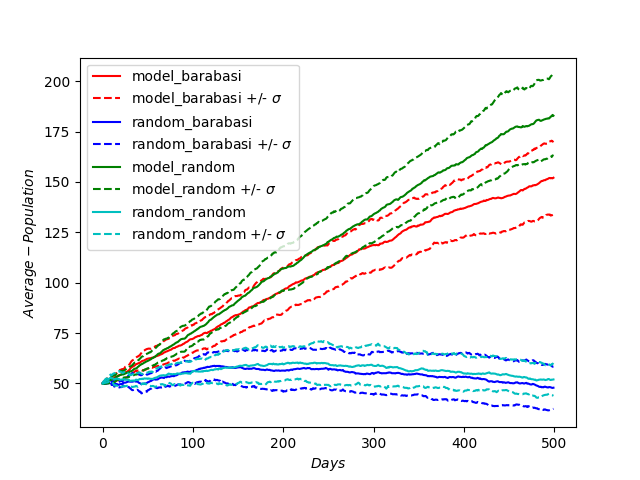
\includegraphics[width=9cm]{images/histories_deviation_price.png}
	\caption{ The history of the node count averages with one standard deviation, for 10 runs. Initially half of the nodes utilizing the generated fee model and the other half a random model. Similarly the attachment strategies are split between Random and Barabasi-Albert. All other strategies are kept equal.
	}
	\label{fig:history_price}
	\hspace*{2mm} 
\end{figure}

\section{Attachment}

The different attachment strategies, excluding biases, were simulated against each other. The results is seen in Figure \ref{fig:history_attachment} 

\begin{figure}[!htb]
	
	\hspace*{-0.5cm}
	\centering
	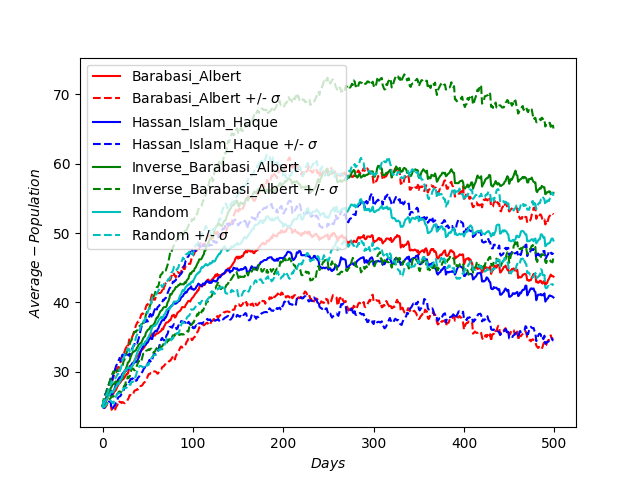
\includegraphics[width=9cm]{images/histories_deviation_attachment.png}
	\caption{ Shows the node count average with one standard deviation for four attachment strategies, Random, Barabasi-Albert, Hassan-Islam-Haque and Inverse-Barabasi for. All else being equal. }
	\label{fig:history_attachment}
	\hspace*{2mm} 
\end{figure}

\section{Funding}

A simulation with four different level of funding was simulated. Each increasing step had twice the funding. The results seen in Figure \ref{fig:funding} suggests that it may be advantageous to be an outlier. Since allocation per channel is equal, this also hints at the optimal amounts of open channels.

However, if the non-advertised nodes would have a fitness attachment selection favoring nodes with high capacity - the well-funded nodes would be highly advantageous as seen in Figure [].  

\newpage

\begin{figure}[!htb]
	\hspace*{-0.7cm}\
	\centering
	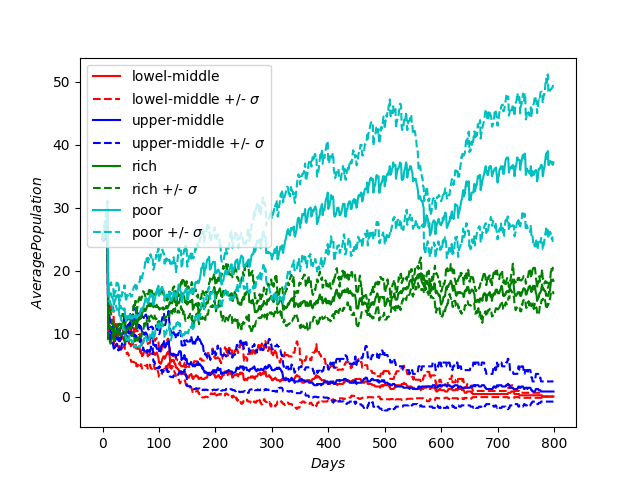
\includegraphics[width=9cm]{images/histories_deviation_fund.png}
	\caption{ Displays the node count and node count average with one standard deviation for four different levels of funding. All other strategies being equal.
	}
	\label{fig:funding}
	\hspace*{2mm} 
\end{figure}

\section{Re-balancing channels}

The two different re-balancing  strategies were tried with various level of aggressiveness. The strategies were first simulated separately and then the best level of aggressiveness of each strategy were simulated again against each other.

\begin{figure}[!htb]
	\hspace*{-0.7cm}\
	\centering
	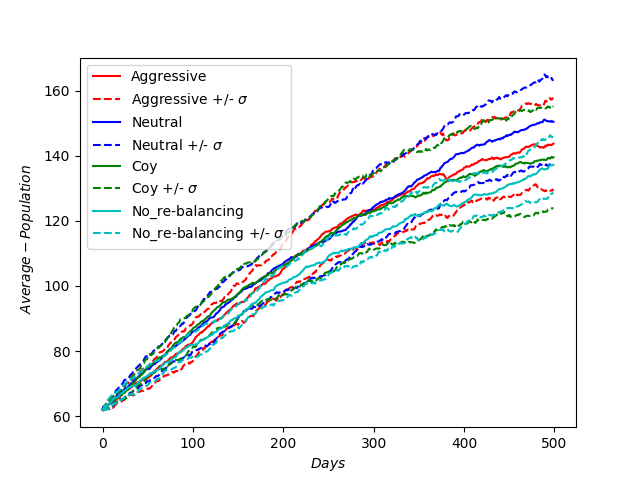
\includegraphics[width=9cm]{images/histories_linear.png}
	\label{fig:linear}
	\hspace*{2mm} 
\end{figure}
\vspace*{-1cm}
\begin{figure}[!htb]
	\hspace*{-0.7cm}\
	\centering
	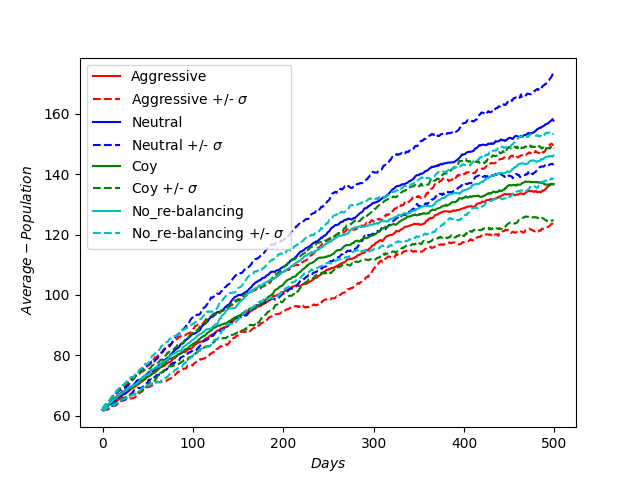
\includegraphics[width=9cm]{images/histories_edge.png}
	\caption{ The above Figure shows the linear displacement strategy with different aggressiveness. While the Figure below shows the edge displacement strategy with different level of bias towards the edge. They look rather similar. They also have a little overall importance, as they all do quite well.
	}
	\label{fig:edge}
	\hspace*{2mm} 
\end{figure}



\begin{figure}[!htb]
	\hspace*{-0.7cm}\
	\centering
	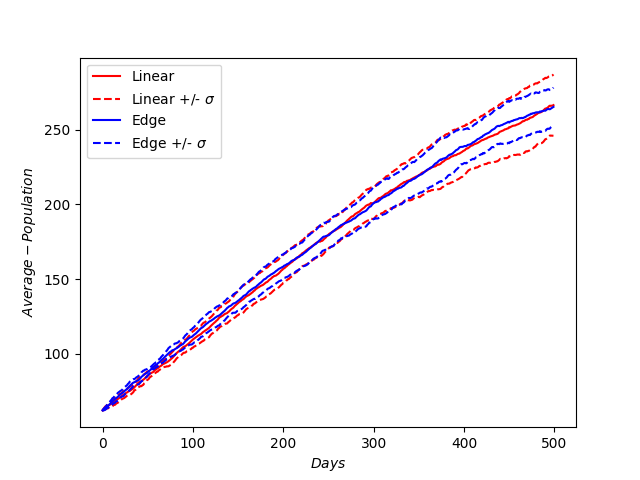
\includegraphics[width=9cm]{images/histories_edge_linear.png}
	\caption{ The above Figure shows the best linear displacement strategy against the best strategy from Figure \ref{fig:edge}.
	}
	\label{fig:funding}
	\hspace*{2mm} 
\end{figure}

\newpage
\section{Revenue distribution}

To explore the innate distribution of the network, only one set of strategies was simulated. Every routing node behaved exactly the same, as it would be the case were the distribution would be expected to be the least extreme. Hence, the extreme tendency here in Figures \ref{fig:path}, \ref{fig:same} suggest that the real distribution would be at least this extreme.   

\begin{figure}[!htb]
	\hspace*{-0.7cm}\
	\centering
	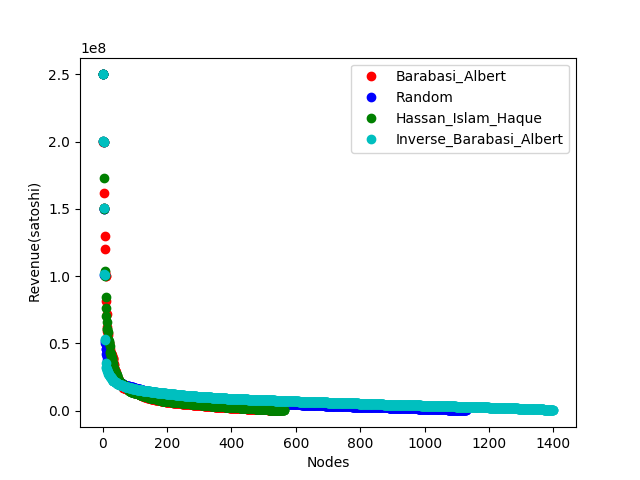
\includegraphics[width=9cm]{images/wealth_distribution_path.png}
	\caption{ Shows the four different simulations separate. Aggregated over two simulations each. Note that environment variables are equal and shows that a broader selection bias supports more nodes. Barabasi-Albert and Hassan-Islam-Haque having a high selection bias towards and few nodes. Random have no bias at al except for time and supports more nodes. Inverse-Barabasi-Albert has an inverse selection bias and subsequently support the most nodes. 
	}
	\label{fig:path}

\end{figure}

\begin{figure}[!htb]
	\vspace{-3cm}
	%\hspace*{-1cm}\
	\centering
	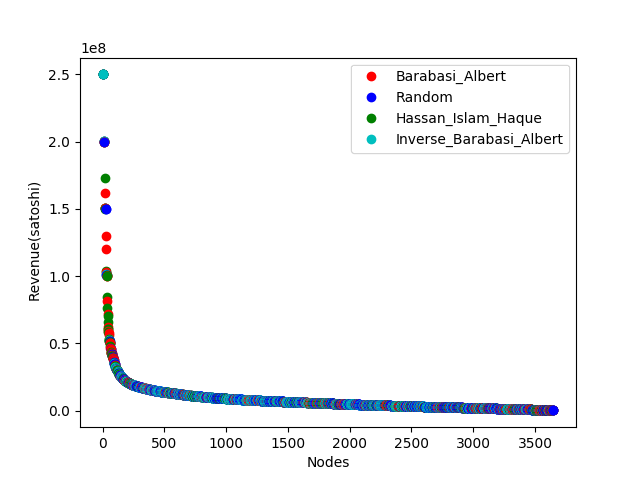
\includegraphics[width=9cm]{images/wealth_distribution_same.png}
	\caption{ Shows
	}
	\label{fig:same}
	\hspace*{2mm} 
\end{figure}

The exponential distribution is akin to previously mentioned Pareto Principle, although in Figures \ref{fig:path}, \ref{fig:same} 20\% of the network account for 60\% of the gross revenue. Note that if profit / net revenue where considered the quotient would be larger. The distribution shown here is in line with the wealth distribution in countries~\cite{credit:swiss:distribution}.

